\documentclass[tikz,border=8pt]{standalone}
\usepackage{amsmath,amssymb}
\usetikzlibrary{arrows.meta,calc,decorations.pathreplacing,patterns,shapes.geometric,positioning,shadings}

\begin{document}
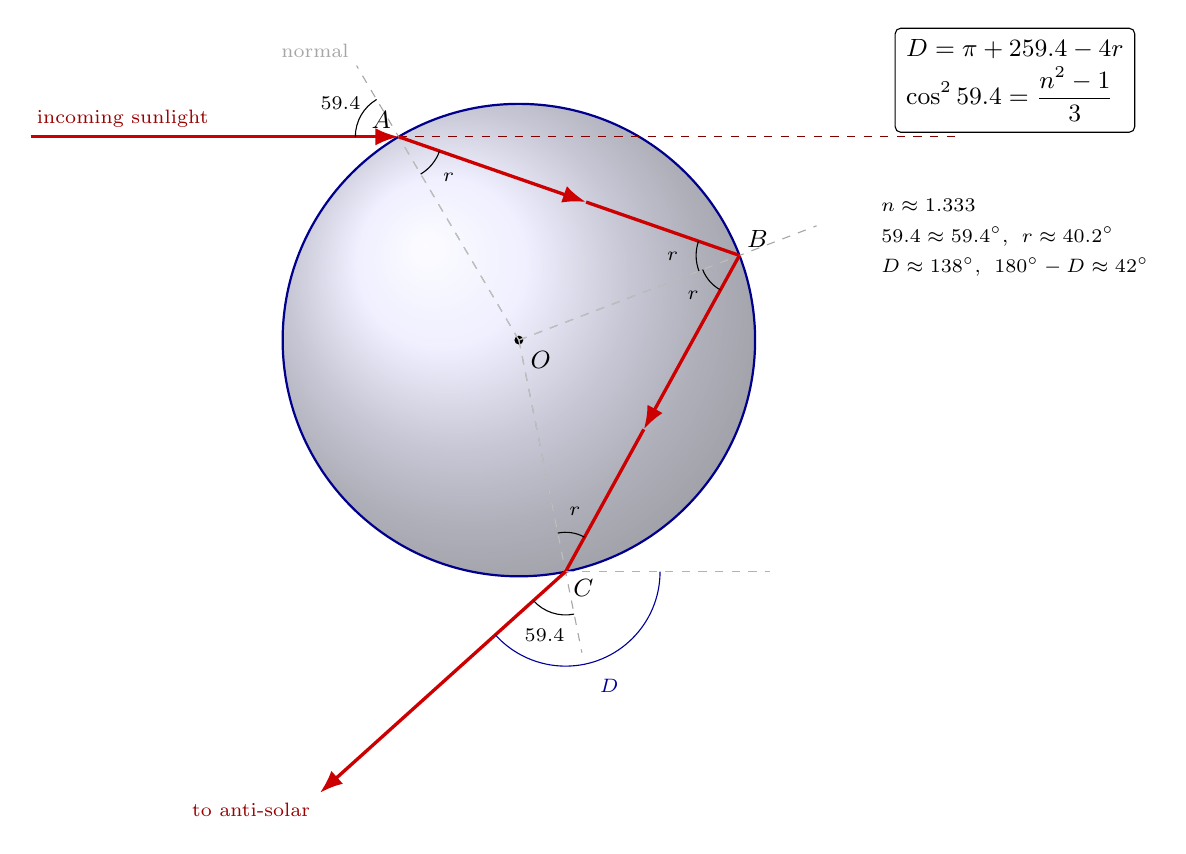
\begin{tikzpicture}[>=Latex, font=\small]

% ---------- Parameters ----------
\def\R{3}             % droplet radius
\def\aA{120.6}        % angular position of A (on circle)
\def\aB{21}           % angular position of B
\def\aC{-78.6}        % angular position of C
\def\theta{59.4}      % incidence angle in degrees
\def\rr{40.2}         % refraction angle inside water

% ---------- Droplet ----------
\shade[ball color=blue!15, opacity=0.55] (0,0) circle (\R);
\draw[thick, blue!55!black] (0,0) circle (\R);

% Center O
\fill (0,0) circle (1.6pt);
\node[below right=1pt] at (0,0) {$O$};

% Points A, B, C on the circle
\coordinate (A) at (\aA:\R);
\coordinate (B) at (\aB:\R);
\coordinate (C) at (\aC:\R);

% Radii / normals (dashed light gray)
\draw[gray!70, dashed] (0,0) -- ($ (A)!-0.35!(0,0) $) node[above left=-1pt] {\scriptsize normal};
\draw[gray!70, dashed] (0,0) -- ($ (B)!-0.35!(0,0) $);
\draw[gray!70, dashed] (0,0) -- ($ (C)!-0.35!(0,0) $);

% Short inward dashes to show radii inside too
\draw[gray!50, dashed] (0,0) -- (A);
\draw[gray!50, dashed] (0,0) -- (B);
\draw[gray!50, dashed] (0,0) -- (C);

% ---------- Rays ----------
% Incoming horizontal ray, at height = y_A, from far left to A
\coordinate (Ain) at (-\R-3.2, {sin(\aA)*\R});
\draw[red!80!black, very thick, ->] (Ain) -- (A);

% Continuation (dashed) of incoming ray through droplet to establish D angle
\coordinate (Acont) at (\R+2.6, {sin(\aA)*\R});
\draw[red!50!black, dashed, thin] (A) -- (Acont);

% Inside segments A -> B -> C
\draw[red!80!black, very thick, ->] (A) -- ($ (A)!0.55!(B) $);
\draw[red!80!black, very thick] ($ (A)!0.55!(B) $) -- (B);
\draw[red!80!black, very thick, ->] (B) -- ($ (B)!0.55!(C) $);
\draw[red!80!black, very thick] ($ (B)!0.55!(C) $) -- (C);

% Outgoing ray from C at angle ~ 222 deg (so that it makes 42 deg with the reversed incoming dir)
\def\outang{222}
\coordinate (Cout) at ($ (C) + (\outang:4.2) $);
\draw[red!80!black, very thick, ->] (C) -- (Cout);

% ---------- Angle labels ----------
% Incidence angle theta at A: between normal (extension outward from A) and incoming ray
% Outward normal at A direction = \aA (degrees); incoming ray approaches from direction \aA+180 reversed...
% For arc labeling, we draw arcs between the outward-normal direction and the reversed-incoming direction at A.
% Reversed incoming (ray points from A back to Ain): angle 180 (pointing -x)
% Outward normal at A: angle \aA = 120.6
% Arc from 180 down to 120.6 spans theta = 59.4 - good.
\draw[thin] ($(A)+(180:0.55)$) arc[start angle=180, end angle=120.6, radius=0.55];
\node at ($(A)+({(180+120.6)/2}:0.85)$) {\scriptsize $\theta$};

% Refraction angle r at A: between inward normal (angle \aA+180 = 300.6) and internal ray AB direction
% AB direction angle: atan2(yB-yA, xB-xA). Compute manually:
%   A=(-1.527, 2.583), B=(2.800, 1.075); AB = (4.327, -1.508); angle = atan2(-1.508, 4.327) ~ -19.2 deg = 340.8 deg
% Inward normal at A: 300.6 deg. Arc from 300.6 to 340.8 spans 40.2 = r. Good.
\draw[thin] ($(A)+(300.6:0.55)$) arc[start angle=300.6, end angle=340.8, radius=0.55];
\node at ($(A)+({(300.6+340.8)/2}:0.82)$) {\scriptsize $r$};

% Refraction angle r at B (on the internal ray arriving): between ray BA direction and inward normal at B
% BA direction at B: from B toward A, angle = atan2(1.508, -4.327) ~ 180-19.2 = 160.8 deg
% Inward normal at B: angle \aB+180 = 201
% Arc from 160.8 to 201 spans ~40.2 = r
\draw[thin] ($(B)+(160.8:0.55)$) arc[start angle=160.8, end angle=201, radius=0.55];
\node at ($(B)+({(160.8+201)/2}:0.85)$) {\scriptsize $r$};

% Another r at B (on reflected side, between inward normal and ray BC)
% BC direction: B=(2.800,1.075), C=(0.591,-2.940); BC=(-2.209,-4.015); angle = atan2(-4.015,-2.209) ~ 180+61.2 = 241.2
% Arc from 201 to 241.2 spans 40.2 = r
\draw[thin] ($(B)+(201:0.5)$) arc[start angle=201, end angle=241.2, radius=0.5];
\node at ($(B)+({(201+241.2)/2}:0.78)$) {\scriptsize $r$};

% r at C (on internal side) and theta at C (on outside exit)
% CB direction at C: angle 241.2 + 180 = 61.2
% Inward normal at C: \aC+180 = 101.4
% Arc from 61.2 to 101.4 spans 40.2 = r
\draw[thin] ($(C)+(61.2:0.5)$) arc[start angle=61.2, end angle=101.4, radius=0.5];
\node at ($(C)+({(61.2+101.4)/2}:0.78)$) {\scriptsize $r$};

% theta at C: outward normal at C angle \aC = -78.6 = 281.4; outgoing ray angle 222
% Arc from 222 to 281.4 spans 59.4 = theta
\draw[thin] ($(C)+(222:0.55)$) arc[start angle=222, end angle=281.4, radius=0.55];
\node at ($(C)+({(222+281.4)/2}:0.85)$) {\scriptsize $\theta$};

% ---------- Total deviation D ----------
% Extend outgoing ray backward until it meets the incoming-ray continuation (which is horizontal through A's level, extended past C region)
% Incoming continuation y = sin(\aA)*\R = 2.583
% Compute intersection of ray from C in direction (222 deg) extended backward (forward along ray = 222, backward = 42)
% Actually we want the intersection with the forward continuation line y=2.583.
% Outgoing ray from C goes at angle 222; going forward from C it drops; going backward from C (angle 42) it rises -
% that meets y=2.583 at some x. Let's compute that intersection to place D arc.
% Point P such that P = C + t*(cos 42, sin 42) with y = -2.94 + t*sin42 = 2.583 => t = (2.583+2.94)/sin42 = 5.523/0.669 = 8.255
% x = 0.591 + 8.255*cos42 = 0.591 + 8.255*0.743 = 0.591 + 6.133 = 6.724
% That would be far off - use a closer point visually via shorter axes. We'll just mark D with an arc at C between outgoing ray (222) and the direction parallel to incoming ray (0 deg).
% Angle between 222 and 0 going clockwise: 222 -> 0 CCW is 138 deg (which equals D). Draw arc at C.
\draw[thin, blue!60!black] ($(C)+(0:1.2)$) arc[start angle=0, end angle=-138, radius=1.2];
\node[blue!60!black] at ($(C)+(-69:1.55)$) {\scriptsize $D$};

% Dashed horizontal reference through C for angle D visualization
\draw[gray!60, dashed, thin] (C) -- ++(2.6,0);

% ---------- Point labels ----------
\node[above left=-1pt] at (A) {$A$};
\node[above right=-1pt] at (B) {$B$};
\node[below right=-1pt] at (C) {$C$};

% Incoming ray label
\node[red!60!black, above] at ($(Ain)!0.25!(A)$) {\scriptsize incoming sunlight};
% Outgoing ray label
\node[red!60!black, below left] at (Cout) {\scriptsize to anti-solar};

% ---------- Formula box (top right) ----------
\node[draw, rounded corners=2pt, fill=white, align=left, inner sep=4pt] at (6.3,3.3)
  {$\displaystyle D = \pi + 2\theta - 4r$\\[2pt]
   $\displaystyle \cos^2\theta = \dfrac{n^2-1}{3}$};

% ---------- Parameters note ----------
\node[align=left] at (6.3,1.3)
  {\scriptsize $n \approx 1.333$\\
   \scriptsize $\theta \approx 59.4^\circ$,\; $r \approx 40.2^\circ$\\
   \scriptsize $D \approx 138^\circ$,\; $180^\circ - D \approx 42^\circ$};

\end{tikzpicture}
\end{document}
